% ============================================================
%  CHAPITRE 2 — Méthodologie et Conception de l'Architecture
%  Mémoire de Master BIBDA — CHOUFA ZOUHAIR
%  Université Chouaib Doukkali — Faculté des Sciences El Jadida
%  Titre : Gestion de l'hétérogénéité des données tabulaires
%          pour la génération de Knowledge Graphs (Big Data + KG)
% ============================================================

\chapter{Méthodologie et Conception de l'Architecture}
\label{chap:methodologie}

% ─────────────────────────────────────────────────────────────
\section{Introduction et Justification des Choix Architecturaux}
\label{sec:intro_methodo}
% ─────────────────────────────────────────────────────────────

L'analyse critique de la littérature conduite au chapitre~\ref{chap:etat_art}
a mis en évidence quatre lacunes structurelles récurrentes dans les approches
existantes de transformation de données tabulaires hétérogènes en Knowledge
Graphs. Premièrement, les approches recensées sont \textbf{fragmentées} :
elles traitent isolément le schema matching, la triplification ou la
résolution d'entités, sans proposer de chaîne de traitement intégrée de
bout en bout. Deuxièmement, elles \textbf{gèrent mal l'hétérogénéité
multi-sources} : la plupart des travaux supposent une source unique ou
des schémas déjà proches, et n'adressent pas explicitement les trois
niveaux d'hétérogénéité (structurelle, syntaxique, sémantique) identifiés
à la section~\ref{sec:construction_auto}. Troisièmement, elles
\textbf{exploitent peu les grands modèles de langage de manière
contrôlée} : lorsqu'un LLM est utilisé, il l'est le plus souvent de
façon systématique et coûteuse, sans stratégie de filtrage préalable ni
mécanisme de validation structurée de ses sorties. Enfin, elles sont
\textbf{rarement reproductibles}, faute d'environnement d'exécution
conteneurisé et de protocole d'évaluation partagé.

Ces observations convergent vers un besoin scientifique et technique précis :
la conception d'un pipeline \textit{unifié}, \textit{déclaratif},
\textit{automatisé} et \textit{reproductible}, dans lequel chaque module est
évaluable indépendamment et l'ensemble est déployable sans intervention
manuelle sur des volumes de données variables.
\textbf{Pour répondre à ces limitations, nous proposons un pipeline composé
de cinq modules fonctionnels séquentiels, complétés par une infrastructure
d'orchestration Docker Compose et un protocole d'évaluation fondé sur un
gold standard annoté manuellement}, détaillé à la
section~\ref{sec:protocole_eval}. Cette continuité directe entre les
lacunes identifiées au chapitre~\ref{chap:etat_art} et les choix de
conception présentés dans ce chapitre en constitue le fil conducteur.

La contribution de ce mémoire répond à ce besoin par la conception et
l'implémentation d'une architecture en cinq modules séquentiels et
interdépendants, orchestrés par Docker Compose.
Cette architecture se distingue des travaux existants par trois apports
principaux.
Premièrement, le \textbf{schema matching est hybride} : il combine un module
symbolique déterministe basé sur les embeddings Sentence-BERT~\cite{reimers2019sbert}
pour les correspondances à haute similarité lexicale, et un agent LLM piloté par
LangChain~\cite{langchain2023} pour les cas ambigus, avec génération automatique
des règles de mapping au format YARRRML~\cite{warren2024yarrrml}.
Deuxièmement, la \textbf{triplification est entièrement déclarative} : les règles
YARRRML sont exécutées par le moteur Morph-KGC~\cite{arenas2023morphkgc}, ce qui
garantit la séparation entre la logique métier de transformation et le code
d'exécution.
Troisièmement, la \textbf{reproductibilité est garantie par la conteneurisation}
complète de la stack via Docker Compose~\cite{docker2024}, rendant le pipeline
déployable en une seule commande sur n'importe quelle infrastructure compatible.

Ce chapitre présente en détail la conception de chacun de ces cinq modules.
Nous commençons par décrire l'architecture globale (section~\ref{sec:archi_globale}),
avant de détailler successivement le module d'ingestion
(section~\ref{sec:module_ingestion}), le module de schema matching hybride
(section~\ref{sec:module_matching}), le module de triplification
(section~\ref{sec:module_triplification}), le module de résolution d'entités et
de validation (section~\ref{sec:module_validation}), et enfin l'orchestration
par Docker Compose (section~\ref{sec:docker}).

% ─────────────────────────────────────────────────────────────
\section{Architecture Globale du Pipeline}
\label{sec:archi_globale}
% ─────────────────────────────────────────────────────────────

La figure~\ref{fig:pipeline_global} présente l'architecture globale du pipeline
proposé.
Celui-ci est organisé comme un flux de données unidirectionnel, allant des sources
hétérogènes brutes jusqu'au Knowledge Graph validé et interrogeable, en passant
par cinq modules fonctionnels distincts.
Chaque module produit un artefact intermédiaire formellement défini, ce qui permet
d'évaluer la qualité de la transformation à chaque étape indépendamment du reste
du pipeline.

% ── FIGURE : Architecture globale ────────────────────────────
%
%  ── CODE MERMAID.JS (commentaire LaTeX) ───────────────────
%  Ce diagramme peut être rendu sur https://mermaid.live
%  en copiant le bloc ci-dessous.
%
%  flowchart LR
%    subgraph SRC ["① Sources Hétérogènes"]
%      S1[CSV / Excel]
%      S2[Base SQL / Dump]
%      S3[JSON / API]
%    end
%
%    subgraph ING ["② Ingestion & Profilage"]
%      I1[Connecteurs\nPython / PySpark]
%      I2[Data Profiling\nydata-profiling]
%      I3[Staging\nMongoDB]
%    end
%
%    subgraph MAT ["③ Schema Matching Hybride"]
%      M1[Embeddings\nSentence-BERT]
%      M2{Score\n≥ seuil ?}
%      M3[Agent LLM\nLangChain]
%      M4[Règles\nYARRRML]
%      M1 --> M2
%      M2 -- Oui --> M4
%      M2 -- Non --> M3
%      M3 --> M4
%    end
%
%    subgraph TRI ["④ Triplification"]
%      T1[Morph-KGC]
%      T2[Triplets RDF\n.nt / .ttl]
%      T1 --> T2
%    end
%
%    subgraph RES ["⑤ Résolution & Validation"]
%      R1[Entity Resolution\nSplink]
%      R2[owl:sameAs]
%      R3[Validation\nSHACL / PySHACL]
%      R1 --> R2
%      R2 --> R3
%    end
%
%    subgraph STO ["⑥ Stockage & Requêtage"]
%      G1[GraphDB\nTriple Store]
%      G2[SPARQL\nEndpoint]
%      G1 --> G2
%    end
%
%    SRC --> ING --> MAT --> TRI --> RES --> STO
%
%    style SRC fill:#f5f5f5,stroke:#999
%    style ING fill:#e8f4fd,stroke:#2E75B6
%    style MAT fill:#e8f5e9,stroke:#2E7D32
%    style TRI fill:#fff3e0,stroke:#E65100
%    style RES fill:#f3e5f5,stroke:#6A1B9A
%    style STO fill:#e8eaf6,stroke:#1565C0
%  ────────────────────────────────────────────────────────────

% \begin{figure}[htbp]
%     \centering
%     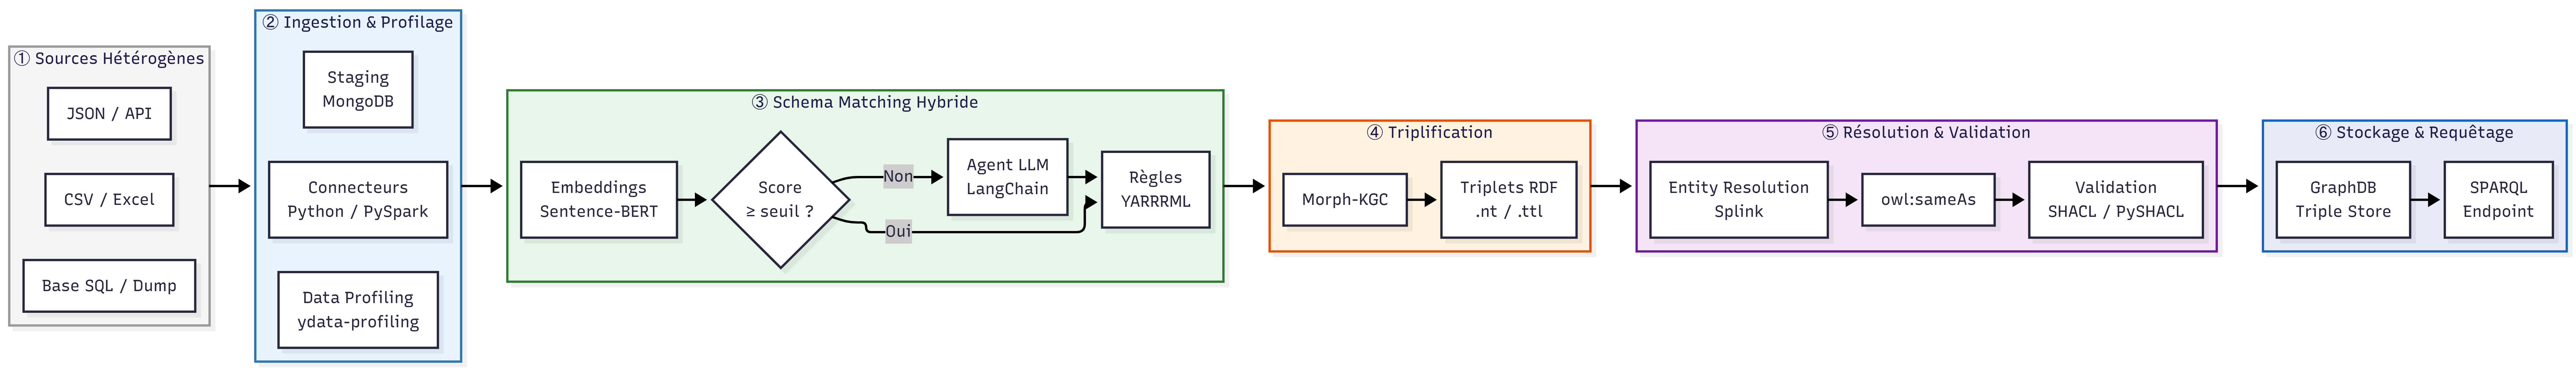
\includegraphics[width=\linewidth]{pics/Heterogeneous Data pipeline global.png}
%     \caption{Heterogeneous Data Pipeline Global}
%     \label{fig:heterogeneous-data-pipeline-global}
% \end{figure}

\begin{figure}[ht]
    \centering
    \resizebox{\textwidth}{!}{
    \begin{tikzpicture}[
        >=latex,
        % Styles des boîtes (textes plus grands grâce au changement d'échelle)
        box/.style    = {draw, rounded corners=5pt, align=center,
                         minimum height=1.2cm, font=\small,
                         text width=2.8cm},
        src/.style    = {box, fill=gray!8,        draw=gray!60},
        ing/.style    = {box, fill=blue!7,        draw=blue!50},
        mat/.style    = {box, fill=green!7,       draw=green!50!black},
        tri/.style    = {box, fill=orange!8,      draw=orange!70!black},
        res/.style    = {box, fill=violet!7,      draw=violet!60},
        sto/.style    = {box, fill=blue!10,       draw=blue!60!black},
        dec/.style    = {diamond, draw=green!50!black, fill=green!7,
                         align=center, font=\footnotesize,
                         inner sep=1pt, aspect=1.5},
        arr/.style    = {->, thick, draw=gray!70},
        % Style des grosses flèches entre les groupes (avec coins arrondis)
        grparr/.style = {->, line width=1.5pt, draw=blue!60, dashed, rounded corners=10pt},
    ]

    %% ════════════════ LIGNE 1 (EN HAUT) ════════════════

    %% ── Colonne 1 : Sources (X = 0) ──
    \node[src] (s1) at (0, 0)    {CSV / Excel};
    \node[src] (s2) at (0, -1.8) {Base SQL\\Dump};
    \node[src] (s3) at (0, -3.6) {JSON / API};

    \node[draw=gray!60, rounded corners, dashed, thick,
          fit=(s1)(s3), inner sep=6pt,
          label={[font=\small\bfseries]above:{\textcircled{1} Sources}}] (grp_src) {};

    %% ── Colonne 2 : Ingestion (X = 4.5) ──
    \node[ing] (i1) at (4.5, 0)    {Profiling\\ydata-profiling};
    \node[ing] (i2) at (4.5, -1.8) {Connecteurs\\Python/PySpark};
    \node[ing] (i3) at (4.5, -3.6) {Staging\\MongoDB};

    \node[draw=blue!50, rounded corners, dashed, thick,
          fit=(i1)(i2)(i3), inner sep=6pt,
          label={[font=\small\bfseries]above:{\textcircled{2} Ingestion}}] (grp_ing) {};

    %% ── Colonne 3 : Schema Matching (X = 9.0 et LLM à 12.8) ──
    \node[mat] (m1) at (9.0, 0)    {Sentence-BERT\\Embeddings};
    \node[dec] (md) at (9.0, -1.8) {Score\\$\geq \tau$ ?};
    \node[mat] (m4) at (9.0, -3.6) {Règles\\YARRRML};
    
    \node[mat] (m3) at (12.8, -1.8) {Agent LLM\\LangChain};

    \node[draw=green!50!black, rounded corners, dashed, thick,
          fit=(m1)(md)(m4)(m3), inner sep=6pt,
          label={[font=\small\bfseries]above:{\textcircled{3} Schema Matching}}] (grp_mat) {};


    %% ════════════════ LIGNE 2 (EN BAS) ════════════════
    
    %% ── Colonne 4 : Triplification (X = 0, Y = -8.0) ──
    \node[tri] (t1) at (0, -8.0) {Morph-KGC\\Moteur RML};
    \node[tri] (t2) at (0, -9.8) {Triplets RDF\\.nt / .ttl};

    \node[draw=orange!70!black, rounded corners, dashed, thick,
          fit=(t1)(t2), inner sep=6pt,
          label={[font=\small\bfseries]above:{\textcircled{4} Triplification}}] (grp_tri) {};

    %% ── Colonne 5 : Résolution (X = 4.5, Y = -8.0) ──
    \node[res] (r1) at (4.5, -8.0)  {Entity Res.\\Splink};
    \node[res] (r2) at (4.5, -9.8)  {\texttt{owl:sameAs}\\Fusion};
    \node[res] (r3) at (4.5, -11.6) {Validation\\SHACL};

    \node[draw=violet!60, rounded corners, dashed, thick,
          fit=(r1)(r2)(r3), inner sep=6pt,
          label={[font=\small\bfseries]above:{\textcircled{5} Résolution}}] (grp_res) {};

    %% ── Colonne 6 : Stockage (X = 9.0, Y = -8.0) ──
    \node[sto] (g1) at (9.0, -8.0) {GraphDB\\Triple Store};
    \node[sto] (g2) at (9.0, -9.8) {SPARQL\\Endpoint};

    \node[draw=blue!60!black, rounded corners, dashed, thick,
          fit=(g1)(g2), inner sep=6pt,
          label={[font=\small\bfseries]above:{\textcircled{6} Stockage}}] (grp_sto) {};


    %% ════════════════ FLUX ENTRE LES GROUPES ════════════════
    \draw[grparr] (grp_src.east) -- (grp_ing.west);
    \draw[grparr] (grp_ing.east) -- (grp_mat.west);
    
    % Flèche magique : relie la fin de la Ligne 1 au début de la Ligne 2
    % Part du Sud du groupe 3, descend, va à gauche jusqu'au groupe 4, puis descend
    \draw[grparr] (grp_mat.south) -- ++(0, -0.8) -| (grp_tri.north);

    \draw[grparr] (grp_tri.east) -- (grp_res.west);
    \draw[grparr] (grp_res.east) -- (grp_sto.west);

    %% ════════════════ FLUX INTERNES ════════════════
    % Schema Matching
    \draw[arr] (m1) -- (md);
    \draw[arr] (md) -- node[above, font=\footnotesize]{Non} (m3);
    \draw[arr] (md) -- node[right, font=\footnotesize]{Oui} (m4);
    \draw[arr] (m3.south) |- (m4.east);

    % Triplification
    \draw[arr] (t1) -- (t2);

    % Résolution
    \draw[arr] (r1) -- (r2);
    \draw[arr] (r2) -- (r3);

    % Stockage
    \draw[arr] (g1) -- (g2);

    \end{tikzpicture}
    } % Fin du resizebox
    
    \vspace{0.4cm}
    \caption{Architecture globale du pipeline de transformation structurée en deux phases. 
             La première ligne illustre l'ingestion et l'alignement sémantique hybride. 
             La seconde ligne détaille la génération RDF, la résolution d'entités et le stockage final.}
    \label{fig:pipeline_global}
\end{figure}



Le pipeline est composé de \textbf{cinq modules fonctionnels} complétés par
une infrastructure d'orchestration transverse (Docker Compose,
section~\ref{sec:docker}). Chaque module répond à une problématique
spécifique de l'intégration de données hétérogènes, et son artefact de
sortie constitue l'artefact d'entrée du module suivant, sans état partagé
implicite entre les étapes.

\begin{itemize}
    \item \textbf{Module 1 — Ingestion et prétraitement}
          (section~\ref{sec:module_ingestion}) : collecte des sources
          brutes hétérogènes (CSV, Excel, SQL, JSON), profilage
          automatique de la qualité, normalisation syntaxique et
          persistance dans une zone de staging MongoDB. Il traite
          exclusivement l'hétérogénéité \textit{structurelle} et
          \textit{syntaxique}.
    \item \textbf{Module 2 — Schema matching hybride}
          (section~\ref{sec:module_matching}) : identification de la
          propriété ontologique correspondant à chaque colonne source,
          par une cascade SBERT (rapide, déterministe) puis agent LLM
          (coûteux, réservé aux cas ambigus), et génération automatique
          des règles de mapping YARRRML. C'est le module qui résout
          l'hétérogénéité \textit{sémantique}, la plus difficile des
          trois.
    \item \textbf{Module 3 — Triplification}
          (section~\ref{sec:module_triplification}) : exécution
          déclarative des règles YARRRML par le moteur Morph-KGC,
          produisant les triplets RDF conformes à l'ontologie cible.
    \item \textbf{Module 4 — Résolution d'entités et validation}
          (section~\ref{sec:module_validation}) : réconciliation
          probabiliste des entités décrites par plusieurs sources
          (Splink), génération des ponts \texttt{owl:sameAs}, puis
          validation structurelle du graphe par des contraintes SHACL.
    \item \textbf{Module 5 — Stockage et requêtage} : chargement du
          graphe validé dans un triple store (GraphDB) exposant un
          point d'accès SPARQL, ainsi qu'une interface de visualisation
          interactive.
\end{itemize}

\noindent L'ensemble de ces modules est orchestré par
\textbf{Docker Compose} (section~\ref{sec:docker}), qui garantit que le
pipeline complet est déployable en une seule commande, indépendamment de
l'infrastructure hôte — répondant directement au déficit de
reproductibilité identifié au chapitre~\ref{chap:etat_art}.

Le tableau~\ref{tab:artefacts} synthétise les artefacts d'entrée et de sortie
de chaque module, matérialisant l'interface contractuelle entre les étapes
successives du pipeline.

\begin{table}[ht]
\centering
\caption{Artefacts d'entrée et de sortie de chaque module du pipeline.}
\label{tab:artefacts}
\renewcommand{\arraystretch}{1.35}
\begin{tabular}{|p{0.5cm}|p{3.2cm}|p{4.2cm}|p{4.2cm}|}
\hline
\textbf{\#} & \textbf{Module} & \textbf{Entrée} & \textbf{Sortie} \\
\hline
1 & Ingestion \& Profilage
  & Fichiers CSV, Excel, dumps SQL, JSON bruts
  & DataFrames normalisés, rapports de profilage,
    collections MongoDB de staging \\
\hline
2 & Schema Matching Hybride
  & Schémas sources (noms et exemples de colonnes),
    ontologie OWL cible
  & Règles de mapping YARRRML validées par module \\
\hline
3 & Triplification
  & Données normalisées + règles YARRRML
  & Fichiers de triplets RDF (format N-Triples \texttt{.nt}
    ou Turtle \texttt{.ttl}) \\
\hline
4 & Résolution d'entités \& Validation
  & Triplets RDF + contraintes SHACL + ontologie OWL
  & Graphe RDF enrichi (\texttt{owl:sameAs}),
    rapport de validation SHACL \\
\hline
5 & Stockage \& Requêtage
  & Graphe RDF validé
  & Repository GraphDB peuplé, endpoint SPARQL opérationnel \\
\hline
\end{tabular}
\end{table}

% ─────────────────────────────────────────────────────────────
\section{Module 1 : Ingestion et Prétraitement des Données}
\label{sec:module_ingestion}
% ─────────────────────────────────────────────────────────────

\subsection{Rôle fonctionnel}

Le module d'ingestion constitue le point d'entrée du pipeline.
Son rôle est de collecter les données brutes provenant de sources hétérogènes,
de les normaliser dans un format interne unifié, d'en évaluer la qualité, et de
les persister dans une zone de staging avant les traitements sémantiques.
Ce module n'effectue aucune transformation sémantique : son périmètre est
strictement limité à l'hétérogénéité \textit{structurelle} et \textit{syntaxique}
telle que définie dans la taxonomie présentée à la section~\ref{sec:construction_auto}.

\subsection{Sources supportées et stratégie de scalabilité}
\label{subsec:sources}

Le pipeline supporte nativement les formats tabulaires les plus
répandus dans les environnements industriels et académiques :
\begin{itemize}
    \item \textbf{Fichiers plats} : CSV (séparateurs variables,
          encodages UTF-8 et Latin-1), Excel (\texttt{.xlsx} et
          \texttt{.xls}), fichiers TSV à tabulations.
    \item \textbf{Bases relationnelles} : connexion via des dumps SQL
          (\texttt{.sql}) ou via des connecteurs SQLAlchemy~\cite{bayer2012sqlalchemy}
          vers PostgreSQL, MySQL et SQLite.
    \item \textbf{Formats semi-structurés} : JSON tabulaire (tableaux
          d'objets), XML avec structure répétitive extractible.
\end{itemize}

\paragraph{Stratégie de scalabilité : bascule Pandas / PySpark.}
Chaque connecteur est implémenté selon une stratégie à deux niveaux,
afin de couvrir un spectre de volumes allant de quelques milliers à
plusieurs millions d'enregistrements :
\begin{itemize}
    \item \textbf{Mode Pandas}~\cite{pandas2020} :
          utilisé lorsque la taille estimée du fichier source est
          inférieure à un seuil configurable (valeur par défaut :
          \textbf{500 Mo} ou \textbf{$10^6$ lignes}).
          Dans ce mode, l'intégralité des données est chargée en
          mémoire vive, ce qui offre les meilleures performances
          pour les petits volumes grâce à la vectorisation NumPy.
    \item \textbf{Mode PySpark}~\cite{zaharia2016spark} :
          activé automatiquement lorsque la taille dépasse le seuil
          ou lorsque le paramètre \texttt{force\_spark=True} est
          positionné dans la configuration du pipeline.
          PySpark traite les données en partitions distribuées,
          permettant de dépasser les contraintes de mémoire d'un
          seul nœud et d'exploiter un cluster multi-nœuds si
          disponible.
\end{itemize}

La détection automatique du mode est réalisée par un module de
\textbf{profilage léger pré-ingestion} : avant le chargement
complet, seules les métadonnées du fichier (taille en octets,
nombre de lignes estimé par échantillonnage des premiers et derniers
blocs) sont lues, ce qui permet de choisir le moteur approprié
sans charger l'ensemble des données en mémoire.
Dans les deux modes, le résultat produit est un
\textit{DataFrame} dont l'interface est unifiée via une couche
d'abstraction, garantissant que les modules aval (profilage,
normalisation, schema matching) sont indépendants du moteur
d'exécution utilisé.

\subsection{Profilage automatique des données}

Dès l'ingestion, chaque source fait l'objet d'un \textbf{profilage automatique}
via la bibliothèque \texttt{ydata-profiling}~\cite{ydataprofiling2023}.
Ce profilage produit pour chaque colonne : son type inféré (numérique, catégoriel,
temporel, textuel), sa cardinalité, son taux de valeurs manquantes, sa
distribution statistique (quartiles, histogramme), et des exemples de valeurs
représentatives.

Ces métadonnées de profilage jouent un rôle crucial dans le module suivant :
elles constituent la \textbf{représentation augmentée de colonne} transmise
au module de schema matching, permettant au module SBERT et à l'agent LLM de
disposer d'un contexte plus riche que le seul nom de la colonne.

\subsection{Staging et Mapping Store dans MongoDB}
\label{subsec:mongodb}

Les DataFrames normalisés sont persistés dans une base
\textbf{MongoDB}~\cite{mongodb2024} utilisée selon deux rôles
complémentaires dans le pipeline.

\paragraph{Rôle 1 — Zone de staging des données.}
MongoDB sert de \textbf{zone de staging intermédiaire} entre le
module d'ingestion et le module de schema matching.
Son schéma flexible (document JSON sans DDL préalable) permet de
stocker des DataFrames de formats hétérogènes dans des collections
séparées, sans migration de schéma.
Chaque collection correspond à une source et contient, en plus
des données normalisées, les métadonnées de profilage
(type inféré, cardinalité, taux de nullité, exemples de valeurs)
sous forme de sous-documents JSON.
Cette co-localisation des données et de leurs métadonnées dans un
même store simplifie l'accès par le module de schema matching,
qui peut requêter simultanément le contenu et le profil d'une
colonne.

\paragraph{Rôle 2 — Mapping Store versionné.}
MongoDB remplit un second rôle, moins courant dans la littérature
mais crucial pour la reproductibilité du pipeline :
il sert de \textbf{mapping store versionné}, c'est-à-dire d'un
référentiel persistant des règles de mapping YARRRML produites
par le module de schema matching.

Chaque règle de mapping est stockée dans une collection dédiée
(\texttt{schema\_mappings}) sous la forme d'un document comprenant :
\begin{itemize}
    \item L'identifiant de la source et le nom de la colonne.
    \item La propriété ontologique cible et le type XSD mappé.
    \item La voie de décision empruntée (\texttt{"sbert"} ou
          \texttt{"llm"}).
    \item Le score de confiance associé.
    \item Un \textbf{horodatage} et un \textbf{identifiant de version}
          permettant de tracer l'historique des modifications.
    \item Un indicateur de validation humaine (\texttt{validated: true/false}).
\end{itemize}

Cette architecture de mapping store présente deux avantages
majeurs.
Premièrement, elle permet de \textbf{réutiliser les règles validées}
lors d'une exécution ultérieure du pipeline sur la même source,
sans relancer le module de schema matching.
Deuxièmement, elle offre un mécanisme de \textbf{révision humaine
incrémentale} : un expert métier peut consulter et valider les
correspondances via une interface dédiée, et les règles invalidées
sont automatiquement soumises à une nouvelle analyse LLM lors de
la prochaine exécution.
Ce paradigme est aligné avec les recommandations
\textit{human-in-the-loop} de la littérature récente sur
l'automatisation du schema matching~\cite{branco2025integration}.

\subsection{Normalisation syntaxique}

Avant la persistance en staging, un module de normalisation syntaxique applique
une série de transformations canoniques sur les valeurs :
\begin{itemize}
    \item \textbf{Dates} : toutes les dates sont converties vers le format
          ISO 8601 (\texttt{YYYY-MM-DD}), indépendamment du format source
          (\texttt{DD/MM/YYYY}, \texttt{MM-DD-YY}, \texttt{Jan 15, 2024},
          etc.), en s'appuyant sur la bibliothèque \texttt{dateutil}~\cite{dateutil2024}.
    \item \textbf{Nombres} : unification des séparateurs décimaux et de milliers,
          suppression des symboles monétaires, conversion vers \texttt{float64}.
    \item \textbf{Textes} : normalisation Unicode (NFC), homogénéisation de la
          casse, suppression des espaces superflus.
    \item \textbf{Valeurs nulles} : détection et remplacement cohérent des
          représentations variées du vide (\texttt{"N/A"}, \texttt{"null"},
          cellule vide, \texttt{"-"}).
\end{itemize}
Ces normalisations syntaxiques réduisent directement l'hétérogénéité de niveau 2
(syntaxique) avant que les données n'atteignent le moteur de triplification, où
elles seront typées explicitement via les types XSD de RDF.

\medskip
Une fois les données ingérées, normalisées et persistées dans la zone de
staging MongoDB, le pipeline dispose d'une représentation structurellement
homogène de sources initialement hétérogènes. La question qui se pose alors
est d'ordre sémantique~: comment identifier automatiquement la propriété
ontologique vers laquelle chaque colonne doit être mappée~? C'est l'objet
du Module~2, présenté dans la section suivante.

% ─────────────────────────────────────────────────────────────
\section{Module 2 : Schema Matching Hybride et Génération YARRRML}
\label{sec:module_matching}
% ─────────────────────────────────────────────────────────────

Ce module constitue le \textbf{cœur scientifique} de la contribution présentée
dans ce mémoire.
Son objectif est de résoudre l'hétérogénéité sémantique --- la plus difficile des
trois formes d'hétérogénéité --- en identifiant automatiquement la correspondance
entre chaque colonne d'une source tabulaire et la propriété ontologique adéquate
de l'ontologie OWL cible, puis en formalisant cette correspondance dans une règle
de mapping YARRRML prête à être exécutée par Morph-KGC.

\subsection{Représentation des colonnes sources}

L'entrée de ce module n'est pas simplement le nom d'une colonne, mais une
\textbf{représentation augmentée} composée de :
\begin{itemize}
    \item Le \textbf{nom de la colonne} (\textit{header}) tel qu'extrait de
          la source.
    \item Le \textbf{type inféré} et la \textbf{distribution statistique} issus
          du profilage (section~\ref{sec:module_ingestion}).
    \item Trois à cinq \textbf{exemples de valeurs} représentatives de la colonne.
    \item Le \textbf{nom de la table source} et, le cas échéant, les noms des
          colonnes adjacentes (contexte structurel local).
\end{itemize}
Cette représentation augmentée permet de discriminer deux colonnes portant le
même nom mais appartenant à des tables de domaines différents (par exemple,
une colonne \texttt{date} dans une table de commandes et une colonne \texttt{date}
dans une table de naissances).

% À insérer comme nouvelle sous-section entre 2.4.1 et 2.4.2
\subsection{L'ontologie du domaine : artefact central du pipeline}
\label{subsec:ontologie}

Avant de décrire le processus d'alignement, il est nécessaire
de préciser la nature et la structure de l'\textbf{ontologie OWL
cible} vers laquelle toutes les colonnes sources sont mappées.
Cette ontologie constitue l'artefact sémantique fondateur du
pipeline : elle définit le vocabulaire partagé qui permet d'unifier
des sources hétérogènes sous un modèle de connaissance commun.

\paragraph{Conception et structure.}
L'ontologie du domaine est modélisée sous
\textbf{Protégé}~\cite{musen2015protege} (version 5.x),
le standard académique et industriel pour la création d'ontologies
OWL 2 DL.
Elle suit le principe de \textbf{réutilisation maximale} :
les classes et propriétés des vocabulaires standards du Web
Sémantique sont réutilisées chaque fois que possible, et
complétées par des éléments spécifiques au domaine préfixés
\texttt{ex:} (\texttt{http://kg.projet.fr/ontology\#}).

Les vocabulaires réutilisés sont les suivants :
\begin{itemize}
    \item \textbf{FOAF} (\textit{Friend of a Friend})~\cite{foaf2014} :
          pour les personnes (\texttt{foaf:Person}),
          leurs noms (\texttt{foaf:familyName},
          \texttt{foaf:firstName}) et leurs emails
          (\texttt{foaf:mbox}).
    \item \textbf{Schema.org}~\cite{guha2016schemaorg} :
          pour les dates de naissance (\texttt{schema:birthDate}),
          les organisations (\texttt{schema:Organization})
          et les transactions (\texttt{schema:Order}).
    \item \textbf{Dublin Core}~\cite{weibel1998dublin} :
          pour les métadonnées descriptives des sources
          (\texttt{dc:title}, \texttt{dc:source}).
\end{itemize}

L'ontologie compte, dans sa version utilisée pour les expériences
de ce travail, \textbf{12 classes}, \textbf{34 propriétés d'objet}
et \textbf{28 propriétés de données}, couvrant les domaines
de la gestion de la relation client (CRM) et des ressources humaines
(RH), qui correspondent aux sources de données utilisées pour
l'évaluation (voir chapitre~\ref{chap:evaluation}).
Elle est exportée au format Turtle (\texttt{.ttl}) et versionnée
dans le dépôt Git du projet.

\paragraph{Alignement avec OWL 2 DL.}
Le profil OWL 2 DL est retenu pour sa garantie de
\textbf{décidabilité du raisonnement}~\cite{hogan2021knowledge} :
un moteur de raisonnement (HermiT~\cite{shearer2008hermit} dans notre cas)
peut déterminer en temps fini toutes les conséquences logiques de
l'ontologie, notamment les relations d'équivalence entre entités
issues de sources différentes déclarées via
\texttt{owl:equivalentProperty} et \texttt{owl:sameAs}.
Cette propriété est exploitée dans le module de résolution d'entités
décrit à la section~\ref{sec:module_validation}.

\subsection{Approche symbolique : embeddings Sentence-BERT}
\label{subsec:sbert}

La première couche du module de matching est une approche
\textbf{symbolique déterministe} basée sur les embeddings
sémantiques produits par le modèle
Sentence-BERT~\cite{reimers2019sbert}.

Plus précisément, nous utilisons le modèle pré-entraîné \\
\texttt{paraphrase-multilingual-MiniLM-L12-v2}, disponible via la
bibliothèque \\ \texttt{sentence-transformers}~\cite{reimers2019sbert}.
Ce choix est motivé par deux critères complémentaires.
D'une part, ce modèle est conçu pour optimiser la similarité cosinus
comme mesure de proximité sémantique, contrairement aux modèles
BERT originaux dont les représentations ne sont pas directement
comparables via cosinus~\cite{reimers2019sbert}.
D'autre part, sa variante multilingue couvre plus de cinquante
langues, ce qui le rend adapté aux contextes industriels dans lesquels
les colonnes sources peuvent être libellées en français, en anglais
ou dans d'autres langues simultanément.

\paragraph{Processus d'encodage et calcul de similarité.}
Le processus est le suivant :
\begin{enumerate}
    \item Chaque colonne source est encodée en un vecteur dense de
          dimension $d = 384$ à partir de sa représentation augmentée
          (nom de la colonne, type inféré, exemples de valeurs).
    \item Chaque propriété de l'ontologie OWL cible est encodée de la
          même façon, en concaténant son URI locale, son
          \texttt{rdfs:label} et son \texttt{rdfs:comment} en une
          seule chaîne textuelle avant l'encodage.
    \item La \textbf{similarité cosinus} entre chaque vecteur de
          colonne source et chaque vecteur de propriété cible est
          calculée, produisant une matrice de scores
          $S \in [0, 1]^{n_s \times n_p}$, où $n_s$ est le nombre de
          colonnes sources et $n_p$ le nombre de propriétés de
          l'ontologie.
    \item Si le score maximal $s^* = \max_j S_{ij}$ pour la
          colonne $i$ dépasse un seuil $\tau$, la correspondance est
          acceptée automatiquement et la règle YARRRML correspondante
          est générée sans intervention du LLM.
\end{enumerate}

\paragraph{Calibration du seuil $\tau$.}
La valeur du seuil $\tau$ est un hyperparamètre critique du module :
une valeur trop basse génère des correspondances incorrectes
(faux positifs), tandis qu'une valeur trop haute renvoie
inutilement des cas simples vers le LLM, augmentant le coût
computationnel. La valeur par défaut retenue pour ce travail est
$\tau = 0.82$, déterminée par une procédure de calibration sur un
\textbf{gold standard annoté manuellement}.

Cette procédure consiste à calculer le F1-score du module SBERT seul
(sans LLM) pour des valeurs de $\tau$ variant entre $0.60$ et $0.95$
par pas de $0.02$, sur l'ensemble d'entraînement du gold standard.
La valeur $\tau = 0.82$ correspond au maximum du F1-score observé sur
cet ensemble, indiquant le meilleur compromis entre précision (peu de
faux positifs) et rappel (peu de cas simples renvoyés inutilement au
LLM). Les résultats complets de cette calibration, incluant la courbe
F1-score en fonction de $\tau$, sont présentés au
chapitre~\ref{chap:evaluation}.

Cette approche déterministe traite efficacement les cas de
correspondance à forte similarité sémantique (par exemple,
\texttt{nom\_complet} $\rightarrow$ \texttt{foaf:name},
\texttt{email\_professionnel} $\rightarrow$ \texttt{foaf:mbox})
avec un coût computationnel négligeable, de l'ordre de la
milliseconde par paire sur un processeur standard, sans appel API
externe.


\subsection{Approche neuronale : agent LLM via LangChain}
\label{subsec:llm_agent}

Pour les colonnes dont le score SBERT est inférieur au seuil $\tau$,
le pipeline délègue la décision à un \textbf{agent LLM} orchestré
par le framework LangChain~\cite{langchain2023}.
Ce sont typiquement les cas d'hétérogénéité sémantique profonde,
où deux termes désignent le même concept sans partager aucun token
lexical (par exemple, \texttt{CA\_annuel}
$\rightarrow$ \texttt{ex:annualRevenue}).

\paragraph{Choix du modèle de langage.}
LangChain est un framework d'orchestration qui abstrait la couche
d'appel au modèle de langage sous-jacent.
Dans ce travail, le modèle utilisé est \textbf{GPT-4o}
(OpenAI)~\cite{openai2024gpt4}, qui présente les avantages
suivants par rapport aux alternatives évaluées
(Mistral-7B-Instruct~\cite{jiang2023mistral} et
LLaMA-3-8B~\cite{touvron2023llama}) :
\begin{itemize}
    \item \textbf{Précision sur les tâches de raisonnement structural} :
          GPT-4o démontre une capacité supérieure à interpréter le
          contexte sémantique d'une colonne à partir d'exemples de
          valeurs, tâche qui requiert un raisonnement combiné sur le
          nom, le type et le contenu de la colonne.
    \item \textbf{Fiabilité du format de sortie JSON} :
          GPT-4o supporte nativement le mode
          \textit{structured output}~\cite{openai2024gpt4},
          qui garantit que la réponse est un objet JSON
          syntaxiquement valide conforme à un schéma prédéfini,
          éliminant les erreurs de parsing.
    \item \textbf{Latence acceptable} :
          le temps de réponse moyen observé est de l'ordre de
          1 à 3 secondes par requête, compatible avec un usage
          en mode batch sur des dizaines à quelques centaines de
          colonnes ambiguës.
\end{itemize}

Il convient de souligner que le coût d'appel API de GPT-4o constitue
la principale limite de cette approche pour des pipelines à très
grand nombre de colonnes.
C'est précisément la raison pour laquelle le LLM n'est sollicité
qu'en dernier recours, après le filtrage par le module SBERT.
L'architecture hybride permet de limiter le nombre d'appels LLM
au strict minimum des cas ambigus.
La conception du pipeline est par ailleurs compatible avec un
remplacement de GPT-4o par un modèle open-source déployé localement
(Mistral ou LLaMA via Ollama~\cite{ollama2024}) pour les contextes
où la confidentialité des données est une contrainte, sans
modification de l'architecture LangChain.

\paragraph{Structure du prompt.}
L'agent LangChain reçoit un prompt structuré en plusieurs sections :
\begin{itemize}
    \item \textbf{Contexte du domaine} : description de l'ontologie
          cible et de ses classes principales.
    \item \textbf{Description de la colonne source} : nom, type,
          distribution statistique, et trois à cinq exemples de
          valeurs représentatives.
    \item \textbf{Propriétés cibles candidates} : liste des propriétés
          de l'ontologie dont le score SBERT se situe entre
          $\tau - 0.15$ et $\tau$ (zone d'ambiguïté), avec leurs
          définitions \texttt{rdfs:label} et \texttt{rdfs:comment}.
    \item \textbf{Exemples \textit{few-shot}} :
          deux à trois exemples de mappings corrects issus du gold
          standard, présentant des cas similaires d'équivalence
          sémantique sans similarité lexicale.
    \item \textbf{Instruction de sortie} :
          spécification du schéma JSON attendu en sortie, comprenant
          la propriété cible retenue, le score de confiance estimé
          (entre 0 et 1), la transformation XSD à appliquer, et une
          justification textuelle en une phrase.
\end{itemize}

\paragraph{Gestion des erreurs et mécanisme de retry.}
La sortie JSON de l'agent est parsée et validée structurellement
avant d'être utilisée pour générer la règle YARRRML correspondante.
En cas d'incohérence (sortie non conforme au schéma JSON attendu
ou propriété cible non reconnue dans l'ontologie), un mécanisme
de \textit{retry} avec reformulation automatique du prompt est
déclenché, avec un maximum de trois tentatives.
Si les trois tentatives échouent, la colonne est marquée comme
\textit{non réconciliée} et consignée dans un rapport d'anomalies
structuré (format JSON) pour révision humaine, incluant le nom
de la colonne, les scores SBERT des candidats proches, et les
sorties brutes des tentatives LLM.


\subsection{Architecture hybride et seuil adaptatif}

La figure~\ref{fig:schema_matching_detail} illustre le flux de décision du
module de schema matching hybride.
L'articulation entre le module SBERT et l'agent LLM constitue une stratégie
de \textbf{cascade de coûts croissants} : le traitement le moins coûteux
(inférence SBERT locale, de l'ordre de la milliseconde par paire) est tenté
en premier, et le traitement le plus coûteux (appel API LLM, de l'ordre de
la seconde par requête) n'est sollicité que pour les cas que le premier
niveau ne peut résoudre avec confiance.

\begin{figure}[ht]
    \centering
    \resizebox{\textwidth}{!}{
    \begin{tikzpicture}[
        >=latex,
        % Styles des boîtes
        box/.style={draw=gray!80, rounded corners=4pt, align=center,
                    minimum height=1.1cm, font=\small,
                    text width=3.2cm},
        dec/.style={diamond, draw=green!60!black, fill=green!8, 
                    align=center, font=\footnotesize, 
                    inner sep=1pt, aspect=1.8},
        arr/.style={->, thick, draw=gray!80},
        % Styles de couleurs spécifiques
        ok/.style ={draw=green!60!black, fill=green!8},
        llm/.style={draw=orange!80!black, fill=orange!8},
        err/.style={draw=red!60, fill=red!8},
    ]
        
        %% ── Nœuds avec coordonnées absolues ──
        
        \node[box]      (col)    at (0, 0)     {Colonne source\\(repr. augmentée)};
        \node[box, ok]  (sbert)  at (4.5, 0)   {Sentence-BERT\\Embedding};
        \node[dec]      (thresh) at (8.5, 0)   {Score\\$s^* \geq \tau$ ?};
        
        % Branche du Haut (Oui)
        \node[box, ok]  (yarrml) at (12.5, 2)  {Règle\\YARRRML};
        
        % Branche du Bas (Non)
        \node[box, llm] (llm)    at (12.5, -2) {Agent LLM\\(LangChain)};
        \node[dec]      (valid)  at (16.5, -2) {JSON\\valide ?};
        
        % Sous-branches de la validation
        \node[box, ok]  (yar2)   at (20.5, 0)  {Règle\\YARRRML};
        \node[box, err] (err)    at (20.5, -4) {Anomalie\\(révision humaine)};

        %% ── Flèches de connexion orthogonales ──
        
        \draw[arr] (col)   -- (sbert);
        \draw[arr] (sbert) -- (thresh);
        
        % Depuis le premier test (Seuil SBERT)
        % |- signifie "aller à la verticale puis à l'horizontale"
        \draw[arr] (thresh.north) |- node[above left, font=\footnotesize, text=green!60!black]{Oui} (yarrml.west);
        \draw[arr] (thresh.south) |- node[below left, font=\footnotesize, text=orange!80!black]{Non} (llm.west);
        
        \draw[arr] (llm) -- (valid);
        
        % Depuis le second test (Validation JSON)
        \draw[arr] (valid.north) |- node[above left, font=\footnotesize, text=green!60!black]{Oui} (yar2.west);
        \draw[arr] (valid.south) |- node[below left, font=\footnotesize, text=red!80]{Non} (err.west);

    \end{tikzpicture}
    } % Fin du resizebox
    
    \vspace{0.3cm}
    \caption{Flux de décision du module de schema matching hybride.
             Le seuil $\tau$ est calibré empiriquement sur le gold standard
             pour maximiser le F1-score global du module.}
    \label{fig:schema_matching_detail}
\end{figure}

\subsection{Génération automatique des règles YARRRML}

Quelle que soit la voie empruntée (SBERT ou LLM), le résultat du module de
matching est une règle de mapping au format \textbf{YARRRML}.
YARRRML (\textit{Yet Another RDF Mapper}), déjà justifié dans
l'état de l'art~\cite{warren2024yarrrml}, est utilisé ici pour deux raisons
complémentaires.
D'une part, sa syntaxe YAML est lisible et modifiable par un expert métier non
informaticien, ce qui facilite la phase de validation humaine des mappings.
D'autre part, YARRRML est compilable vers des fichiers RML standard, exécutables
par le moteur Morph-KGC sans modification supplémentaire.

Un exemple de règle YARRRML générée automatiquement par le pipeline pour une
source de données clients est présenté ci-dessous :

\begin{verbatim}
prefixes:
  ex:   "http://kg.projet.fr/ontology#"
  foaf: "http://xmlns.com/foaf/0.1/"
  xsd:  "http://www.w3.org/2001/XMLSchema#"

mappings:
  clients_source_A:
    sources: [["clients_A.csv~csv"]]
    s: ex:Customer_$(ID_Client)
    po:
      - [rdf:type, foaf:Person]
      - [foaf:familyName, $(nom_complet), xsd:string]
      - [foaf:mbox, $(email_pro), xsd:anyURI]
      - [ex:annualRevenue, $(CA_annuel), xsd:decimal]
      - [schema:birthDate, $(dt_naissance), xsd:date]
\end{verbatim}

Chaque triplet \texttt{po} (Predicate-Object) est la traduction directe d'une
correspondance identifiée par le module de schema matching : la colonne source
(\texttt{\$(nom\_complet)}) est associée à la propriété ontologique
(\texttt{foaf:familyName}) avec son type XSD cible (\texttt{xsd:string}).

% ─────────────────────────────────────────────────────────────
\section{Module 3 : Triplification Sémantique avec Morph-KGC}
\label{sec:module_triplification}
% ─────────────────────────────────────────────────────────────

\subsection{Rôle fonctionnel}

Le module de triplification transforme les données normalisées en
staging, guidé par les règles YARRRML produites par le module précédent,
en un ensemble de \textbf{triplets RDF} conformes à l'ontologie cible.
C'est l'étape qui matérialise concrètement le passage de la représentation
tabulaire à la représentation graphe.

\subsection{Justification du choix de Morph-KGC}

Le moteur retenu pour l'exécution des règles RML est
\textbf{Morph-KGC}~\cite{arenas2023morphkgc}, développé en Python par
l'équipe d'Arenas-Guerrero et al. (ESWC 2023).
Ce choix est justifié par plusieurs arguments complémentaires par rapport
aux alternatives disponibles (RMLMapper en Java, RDFLib-applet en Python,
triplification manuelle par script).

Premièrement, Morph-KGC est nativement intégrable dans un pipeline Python
sans dépendance JVM, ce qui simplifie l'environnement d'exécution Docker.
Deuxièmement, il supporte les \textbf{fonctions de transformation définies
par l'utilisateur} (\textit{user-defined functions}, UDFs), permettant
d'appliquer des transformations syntaxiques complexes (nettoyage de chaînes,
normalisation de dates, casting de types) directement dans les règles RML,
sans prétraitement séparé.
Troisièmement, sa conception orientée flux (\textit{streaming}) lui permet
de traiter de grands volumes de données sans charger l'intégralité du jeu
de données en mémoire, répondant ainsi à la contrainte de scalabilité
Big Data~\cite{arenas2023morphkgc}.
Quatrièmement, par rapport à un script Python natif utilisant directement
la bibliothèque RDFLib~\cite{rdflib2022}, l'approche déclarative de
Morph-KGC sépare la logique de transformation du code d'exécution :
modifier une règle de mapping ne nécessite pas de modifier le code Python
du pipeline, ce qui améliore la maintenabilité et la testabilité.

\subsection{Processus d'exécution}

L'exécution de Morph-KGC est pilotée par un fichier de configuration INI
qui référence les sources de données, les fichiers de règles YARRRML compilés
en RML, et le format de sortie souhaité.
Deux formats de sortie sont supportés dans notre pipeline :
\begin{itemize}
    \item \textbf{N-Triples} (\texttt{.nt}) : un triplet par ligne, format
          optimal pour le traitement en flux et l'import dans les triple stores.
    \item \textbf{Turtle} (\texttt{.ttl}) : format plus compact et lisible
          par un humain, utilisé pour l'inspection manuelle et la documentation.
\end{itemize}

\subsection{Gestion des graphes nommés}

Pour maintenir la \textbf{traçabilité de la provenance} des triplets générés
depuis des sources multiples, Morph-KGC est configuré pour produire des
\textbf{N-Quads} (\texttt{.nq}) plutôt que des N-Triples lors du traitement
multi-sources.
Chaque triplet est associé à un graphe nommé correspondant à la source dont il
est issu (par exemple,\\  \texttt{<http://kg.projet.fr/graph/source\_A>}).
Cette granularité de provenance facilite l'audit de qualité et la détection
d'incohérences inter-sources dans l'étape suivante.

\medskip
À l'issue de la triplification, le graphe RDF produit est sémantiquement
conforme à l'ontologie cible au niveau des propriétés individuelles. Il
peut cependant contenir deux classes de défauts résiduels~: des entités
redondantes issues de sources multiples représentant le même individu réel,
et des violations de contraintes structurelles définies par l'ontologie. Le
Module~4, présenté dans la section suivante, adresse ces deux classes de
défauts de manière séquentielle et complémentaire.

% ─────────────────────────────────────────────────────────────
\section{Module 4 : Résolution d'Entités et Validation SHACL}
\label{sec:module_validation}
% ─────────────────────────────────────────────────────────────

Ce module opère en deux phases distinctes mais complémentaires :
la résolution d'entités, qui fusionne les représentations redondantes d'une
même entité du monde réel issues de sources différentes, et la validation SHACL,
qui vérifie la conformité formelle du graphe produit à l'ontologie cible.

\subsection{Phase 1 — Résolution d'entités avec Splink}

\subsubsection{Problématique}
Après triplification, le graphe contient potentiellement plusieurs nœuds RDF
distincts représentant la même entité réelle.
Par exemple, le client \textit{Jean Dupont} peut apparaître sous l'URI
\texttt{ex:Customer\_42} issue du système CRM et sous l'URI
\texttt{ex:Customer\_E17} issue du système RH, avec des attributs partiellement
redondants et partiellement complémentaires.
La résolution d'entités (\textit{entity resolution} ou \textit{record linkage})
vise à identifier ces paires et à les fusionner sémantiquement.

\subsubsection{Approche : Splink}
Le pipeline utilise la bibliothèque \textbf{Splink}~\cite{splink2023},
développée par le Ministère de la Justice britannique, pour la résolution
d'entités probabiliste.
Splink implémente le modèle de Fellegi-Sunter~\cite{fellegi1969theory},
dans lequel chaque paire de candidats à la fusion reçoit un score de
correspondance calculé à partir d'une combinaison pondérée de comparaisons
attribut par attribut.

Le processus comporte trois étapes :
\begin{enumerate}
    \item \textbf{Blocking} : pour éviter la comparaison cartésienne de toutes
          les paires possibles (complexité $O(n^2)$), un mécanisme de
          \textit{blocking} regroupe les enregistrements candidats selon des
          clés de blocage (par exemple, première lettre du nom de famille,
          code postal).
          Seules les paires au sein d'un même bloc sont comparées,
          réduisant drastiquement le nombre de comparaisons.
    \item \textbf{Scoring} : pour chaque paire candidate, Splink calcule un
          score de correspondance basé sur des comparaisons multi-attributs :
          similarité de Jaro-Winkler~\cite{winkler1990string} sur les noms,
          correspondance exacte sur les emails, distance de Levenshtein sur
          les adresses.
    \item \textbf{Classification} : les paires dont le score dépasse un seuil
          de décision $\lambda$ (calibré sur le gold standard) sont classifiées
          comme \textit{match} (même entité réelle) et génèrent un triplet
          \texttt{owl:sameAs} reliant leurs deux URIs dans le graphe.
\end{enumerate}

\subsubsection{Génération des triplets \texttt{owl:sameAs}}
Chaque paire classifiée comme \textit{match} produit le triplet RDF suivant,
qui est ajouté au graphe :

\begin{center}
\texttt{<ex:Customer\_42> owl:sameAs <ex:Customer\_E17>}
\end{center}

Ce triplet est exploitable par les raisonneurs OWL : grâce à la sémantique de
\texttt{owl:sameAs}, tout raisonneur peut inférer automatiquement que toutes les
propriétés de \texttt{ex:Customer\_42} s'appliquent aussi à
\texttt{ex:Customer\_E17} et vice versa, créant une vue unifiée et complète de
l'entité sans duplication physique des triplets.

\subsection{Phase 2 — Validation SHACL avec PySHACL}

\subsubsection{Rôle de SHACL dans le pipeline}
La validation SHACL (\textit{Shapes Constraint Language})~\cite{knublauch2017shacl}
est la dernière barrière de qualité avant le chargement du graphe dans le triple
store.
Elle vérifie que chaque entité du graphe respecte les contraintes définies dans
les \textit{shapes} SHACL de l'ontologie cible : cardinalités (une personne doit
avoir exactement un identifiant), types de valeurs (le champ \texttt{birthDate}
doit être de type \texttt{xsd:date}), et patterns d'URIs (les URIs des clients
doivent respecter le patron \texttt{ex:Customer\_[0-9]+}).

\subsubsection{Implémentation avec PySHACL}
La bibliothèque Python \textbf{PySHACL}~\cite{pyshacl2020} est utilisée pour
exécuter la validation.
Elle produit un rapport de conformité structuré listant, pour chaque violation
détectée : le nœud RDF en infraction, la contrainte SHACL violée, et le message
d'erreur associé.

Trois niveaux de sévérité sont distingués dans notre pipeline :
\begin{itemize}
    \item \textbf{Violations bloquantes} (\textit{Violation}) : arrêtent le
          pipeline et empêchent le chargement dans le triple store.
          Exemple : un nœud de type \texttt{foaf:Person} sans propriété
          \texttt{foaf:mbox}.
    \item \textbf{Avertissements} (\textit{Warning}) : consignés dans le rapport
          mais n'empêchent pas le chargement.
          Exemple : une propriété optionnelle absente.
    \item \textbf{Informations} (\textit{Info}) : traces de qualité non critiques.
\end{itemize}

% ─────────────────────────────────────────────────────────────
\section{Orchestration et Reproductibilité : Docker et Big Data}
\label{sec:docker}
% ─────────────────────────────────────────────────────────────

\subsection{Motivation : de la reproductibilité à l'industrialisation}

L'une des limites structurelles des travaux existants identifiées au
chapitre~\ref{chap:etat_art} est la \textbf{reproductibilité insuffisante} des
pipelines publiés, souvent dépendants d'environnements logiciels non documentés
et de données propriétaires.
L'orchestration de l'intégralité de la stack applicative par
\textbf{Docker Compose}~\cite{docker2024} répond directement à cette limite :
elle garantit qu'un tiers peut reproduire exactement l'environnement d'exécution
en une seule commande, sur n'importe quelle machine disposant de Docker Engine,
sans aucune configuration manuelle.

\subsection{Architecture Docker Compose}

La stack complète est définie dans un fichier \texttt{docker-compose.yml}
qui orchestre cinq services conteneurisés :

\begin{enumerate}
    \item \textbf{Service \texttt{python-pipeline}} : le conteneur principal,
          construit à partir d'une image \texttt{python:3.11-slim} via un
          Dockerfile optimisé (cache des couches, ordre de copie, variables
          d'environnement de connexion injectées).
          Il exécute séquentiellement les modules 1 à 4 du pipeline.
    \item \textbf{Service \texttt{mongo}} : instance MongoDB 7.0 pour la zone
          de staging.
          Volume nommé \texttt{mongodb-data} pour la persistance des collections
          entre les redémarrages.
    \item \textbf{Service \texttt{neo4j}} : instance Neo4j 5.x avec le plugin
          \textit{neosemantics} (n10s) pour l'import RDF et les requêtes Cypher
          analytiques.
    \item \textbf{Service \texttt{graphdb}} : instance GraphDB 10.x (Ontotext)
          servant de triple store principal, exposant un endpoint SPARQL 1.1
          sur le port 7200.
    \item \textbf{Service \texttt{streamlit-dashboard}} : interface web de
          visualisation interactive du KG, développée avec
          Streamlit~\cite{streamlit2023} et PyVis pour le rendu graphe.
\end{enumerate}

\subsection{Réseau interne et résolution DNS}

Tous les services partagent un réseau Docker Bridge nommé
\texttt{kg-network}.
Docker fournit automatiquement une résolution DNS interne : le service Python
se connecte à MongoDB via l'URI \texttt{mongodb://mongo:27017} et à GraphDB
via \texttt{http://graphdb:7200}, où \texttt{mongo} et \texttt{graphdb}
sont les noms des services déclarés dans le fichier Compose.
Aucune adresse IP n'est codée en dur, garantissant la portabilité de la
configuration.

\subsection{Gestion des dépendances de démarrage}

Le service \texttt{python-pipeline} ne démarre qu'après que les services
\texttt{mongo} et \texttt{graphdb} ont signalé un état \textit{healthy},
grâce à la directive \texttt{depends\_on} couplée à des
\textbf{healthchecks} Docker.
Le healthcheck de MongoDB interroge la commande \texttt{db.adminCommand('ping')} ;
celui de GraphDB interroge l'endpoint REST \texttt{/rest/repositories} et
attend un code HTTP 200.
Ce mécanisme élimine les problèmes de \textit{race condition} au démarrage
de la stack.

\subsection{Persistance des données et volumes}

Quatre volumes nommés Docker garantissent que les données survivent aux
redémarrages des conteneurs :
\begin{itemize}
    \item \texttt{mongodb-data} : collections de staging et mapping store.
    \item \texttt{graphdb-data} : repository du KG dans GraphDB.
    \item \texttt{neo4j-data} et \texttt{neo4j-import} : graphe Neo4j et
          répertoire d'import de fichiers RDF.
\end{itemize}
La commande \texttt{docker compose down} préserve ces volumes ;
seule la commande \texttt{docker compose down -v} les supprime,
constituant ainsi une commande de remise à zéro explicite et intentionnelle.

\subsection{Justification Big Data de la conteneurisation}

Au-delà de la reproductibilité, l'approche Docker Compose présente un avantage
architectural important dans un contexte Big Data : elle permet de faire
\textbf{évoluer indépendamment} chaque composant du pipeline.
Le service de triplification (Morph-KGC) peut être remplacé par une version
distribuée sur un cluster Spark sans modifier les autres services.
Le triple store GraphDB peut être remplacé par Apache Jena Fuseki ou
Amazon Neptune selon les contraintes de déploiement.
Cette modularité par services est alignée avec les principes des architectures
microservices et avec les patterns d'ingénierie recommandés pour les pipelines
Big Data en production.

% ─────────────────────────────────────────────────────────────
\section{Protocole d'Évaluation et Constitution du Gold Standard}
\label{sec:protocole_eval}
% ─────────────────────────────────────────────────────────────

\subsection{Nécessité d'un gold standard annoté}

L'évaluation quantitative d'un pipeline de transformation vers KG
soulève une difficulté méthodologique spécifique : contrairement
aux tâches de classification supervisée classiques, il n'existe pas
de dataset d'évaluation universel pour le schema matching
multi-sources dans un contexte tabulaire hétérogène.
Les benchmarks communautaires disponibles, tels que
SemTab~\cite{semtab2024, semtab2023}, ciblent des tâches
d'annotation sémantique alignées sur Wikidata, qui ne correspondent
pas exactement à notre cadre (alignement vers une ontologie de domaine
privée).
En cohérence avec les recommandations méthodologiques de la
littérature~\cite{wu2023comprehensive}, nous avons donc constitué
un \textbf{gold standard annoté manuellement}, spécifique au
jeu de données et à l'ontologie utilisés dans ce travail.

\subsection{Constitution du gold standard}

Le gold standard est constitué de \textbf{N paires annotées}
(colonne source, propriété ontologique cible), réparties sur les
deux sources de données hétérogènes utilisées pour l'évaluation
(détaillées au chapitre~\ref{chap:evaluation}).
Chaque paire est annotée par \textbf{deux annotateurs indépendants}
(l'auteur du présent travail et son encadrant académique),
selon une procédure en trois étapes :
\begin{enumerate}
    \item \textbf{Annotation indépendante} :
          chaque annotateur associe chaque colonne à la propriété
          ontologique qu'il juge la plus appropriée, ou à la valeur
          spéciale \texttt{NULL} si aucune propriété ne correspond.
    \item \textbf{Calcul du coefficient d'accord inter-annotateurs}
          (Cohen's Kappa~\cite{cohen1960kappa}) :
          un $\kappa \geq 0.80$ est retenu comme seuil d'acceptabilité,
          indiquant un accord substantiel à excellent.
    \item \textbf{Résolution des désaccords} :
          les cas de divergence ($\kappa < 0.80$ localement) sont
          résolus par discussion et consensus entre les deux
          annotateurs, les décisions étant documentées dans le
          rapport d'annotation.
\end{enumerate}

\subsection{Métriques d'évaluation par module}

Chaque module du pipeline est évalué indépendamment
sur les métriques standard de la littérature :
\begin{itemize}
    \item \textbf{Module de schema matching} :
          Précision ($P$), Rappel ($R$) et F1-score ($F_1$)
          calculés sur les correspondances prédites par rapport
          aux correspondances du gold standard.
    \item \textbf{Module de résolution d'entités} :
          Précision, Rappel et F1-score calculés sur les paires
          \texttt{owl:sameAs} prédites par rapport aux paires
          correctes annotées manuellement.
    \item \textbf{Module de validation SHACL} :
          taux de violations bloquantes détectées sur le graphe
          final (\textit{violation rate}), et taux de conformité
          global (\textit{compliance rate}).
\end{itemize}

Les résultats obtenus sur ces métriques sont présentés et analysés
en détail au chapitre~\ref{chap:evaluation}.

% ─────────────────────────────────────────────────────────────
\section{Conclusion du Chapitre}
\label{sec:conclusion_methodo}
% ─────────────────────────────────────────────────────────────

Ce chapitre a présenté en détail l'architecture et la conception
de chacun des modules du pipeline proposé pour la transformation
de données tabulaires hétérogènes en Knowledge Graph.
L'architecture retenue se distingue des approches de la littérature
identifiées au chapitre~\ref{chap:etat_art} par quatre propriétés
fondamentales.

\textbf{L'automatisation de bout en bout.}
Depuis l'ingestion des fichiers bruts jusqu'au chargement dans le
triple store, aucune intervention manuelle n'est requise dans le
chemin nominal d'exécution.
Les cas ambigus non résolus automatiquement sont systématiquement
signalés dans des rapports d'anomalies structurés, préservant la
transparence du pipeline sans le bloquer.

\textbf{L'hybridation symbolique/neuronale à coûts contrôlés.}
Le module de schema matching combine la rapidité et le déterminisme
de SBERT avec la capacité de raisonnement contextuel des LLMs via
LangChain, dans une architecture en cascade qui maîtrise le coût
computationnel global en limitant les appels API aux seuls cas
ambigus.

\textbf{La conformité aux standards W3C.}
Chaque artefact produit par le pipeline (règles YARRRML, triplets
RDF, contraintes SHACL, triplets \texttt{owl:sameAs}) est conforme
aux standards du Web Sémantique, garantissant l'interopérabilité
avec n'importe quel outil de l'écosystème RDF.

\textbf{La reproductibilité par la conteneurisation.}
L'orchestration Docker Compose rend le pipeline déployable en une
commande sur n'importe quelle infrastructure disposant de Docker
Engine, répondant directement à la lacune de reproductibilité
identifiée dans la littérature.

Il convient cependant de noter que certains paramètres du pipeline
— notamment le seuil $\tau$ du module SBERT, le seuil $\lambda$ du
module Splink, et le nombre d'exemples \textit{few-shot} fournis
à l'agent LLM — constituent des hyperparamètres dont la valeur
optimale est dépendante du domaine.
La méthode de calibration de ces hyperparamètres sur le gold standard
ainsi que leur sensibilité sont analysées au
chapitre~\ref{chap:evaluation}, qui présente également les résultats
expérimentaux complets du pipeline sur le jeu de données hétérogène
retenu pour l'évaluation.